% Unofficial Yale Poster template.
% A fork of the UMich template https://www.overleaf.com/latex/templates/university-of-michigan-umich-poster-template/xpnqzzxwbjzc
% which is fork of the MSU template https://www.overleaf.com/latex/templates/an-unofficial-poster-template-for-michigan-state-university/wnymbgpxnnwd
% which is a fork of https://www.overleaf.com/latex/templates/an-unofficial-poster-template-for-new-york-university/krgqtqmzdqhg
% which is a fork of https://github.com/anishathalye/gemini
% also refer to https://github.com/k4rtik/uchicago-poster



\documentclass[final]{beamer}

% ====================
% Packages
% ====================

\usepackage[T1]{fontenc}
 \usepackage[utf8]{luainputenc}
\usepackage{lmodern}
\usepackage[size=custom, width=122,height=91, scale=1.2]{beamerposter}
\usetheme{gemini}
\usecolortheme{msu}
\usepackage{graphicx}
\usepackage{booktabs}
\usepackage{tikz}
\usepackage{pgfplots}
\pgfplotsset{compat=1.14}
\usepackage{anyfontsize}

% ====================
% Lengths
% ====================

% If you have N columns, choose \sepwidth and \colwidth such that
% (N+1)*\sepwidth + N*\colwidth = \paperwidth
\newlength{\sepwidth}
\newlength{\colwidth}
\setlength{\sepwidth}{0.025\paperwidth}
\setlength{\colwidth}{0.3\paperwidth}

\newcommand{\separatorcolumn}{\begin{column}{\sepwidth}\end{column}}

% ====================
% Title
% ====================

\title{Modeling the Probability of Sufficient Data for Graphical Lasso Maximum Likelihood Estimates }

\author{Hayden Outlaw, Dr. Daniel Bernstein}

\institute[shortinst]{Tulane University}

% ====================
% Footer (optional)
% ====================

\footercontent{
  \href{https://outlawhayden.github.io}{Site: https://outlawhayden.github.io} \hfill
SIAM Algebraic Geometry 2023 Eindhoven \hfill
  \href{mailto:youremail@yale.edu}{houtlaw@tulane.edu}}
% (can be left out to remove footer)

% ====================
% Logo (optional)
% ====================

% use this to include logos on the left and/or right side of the header:
% Left: institution
 \logoright{
\includegraphics[height=8cm]{logos/logo.png}}
% Right: funding agencies and other affilations 
%\logoright{\includegraphics[height=7cm]{logos/NSF.eps}}
% ====================
% Body
% ====================

\begin{document}



\begin{frame}[t]
\begin{columns}[t]
\separatorcolumn

\begin{column}{\colwidth}

    \begin{exampleblock}{Abstract}
    
    Associated to each graph $G$ is a Gaussian graphical model. Such models are often used in high-dimensional settings, i.e. where there are relatively few data points compared to the number of variables. The maximum likelihood threshold of a graph is the minimum number of data points required to fit the corresponding graphical model using maximum likelihood estimation. Graphical lasso is a method for selecting and fitting a graphical model. In this project, we ask: when graphical lasso is used to select and fit a graphical model on $n$ data points, how likely is it that $n$ is greater than or equal to the maximum likelihood of the corresponding graph? 

    \end{exampleblock}

  \begin{block}{Introduction}
Given a sample from a multivariate centered Gaussian distribution $\mathcal{N}(0, \Sigma)$, the covariance matrix of the distribution $\Theta$ can be estimated using maximum likelihood estimation. The covariance can be encoded within a Gaussian graphical model given its sparsity pattern \cite{dempster1981estimation}, and from this model, one can find the minimum number of samples such that the maximum likelihood estimator $\hat{\Theta}_{MLE}$ exists with probability 1 \cite{gross2018maximum}, denoted as the maximum likelihood threshold (MLT).

This is in contrast to the graphLasso covariance estimator, which exists for the same context of selecting and fitting graphical models under centered multi-normal distributions. This estimator is the optimum of the Gaussian log likelihood function with an added $\ell_{1}$ norm penalization. However, when the number of samples is less than the number of parameters in the data, the graphLasso estimator could exist, even if the equivalent maximum likelihood threshold for the same samples and distribution is not met.

I aim to numerically describe, given a sample $S$ of size $n$ from a multivariate normal distribution, the probability that graphLasso estimator $\hat{\Theta}_{GL}$ has a MLT less than or equal to $n$.
  \end{block}

  \begin{block}{Background}
Given a sample $X_1, X_2, \dots, X_n \sim \mathcal{N}(0, \Sigma)$, with a sample covariance $S$, and a penalizing parameter $\alpha$, the graphLasso estimator for the inverse covariance matrix $\Theta = \Sigma^{-1}$ is defined to be \[
\hat{\Theta}_{GL} = argmin_{\Theta \geq 0}(tr(S\Theta) - logdet(\Theta) + \alpha \sum_{j \neq k}|\Theta_{jk}|)
\]\cite{friedman2008sparse}. This function is convex, and can be solved numerically through a wide variety of optimization strategies. 

For the vast majority of contexts, the only information on the MLT is an upper bound. However, for multi-normal distributions of dimension $9$ or less, a calculation for the explicit MLT value can be done for any given sample. Therefore, by numerically sampling from one of these distributions and calculating the MLT, then checking that against the size of the sample, the probability that the number of samples is greater than or equal to the MLT can be bootstrapped, and the behavior of that probability distribution can be modeled numerically. 
  \end{block}

  \begin{block}{Methods}
For a given covariance estimate matrix $S$, the underlying model structure can be represented as a graph $G = (V, E)$. From Bernstein et al., \cite{bernstein2022computing}, the MLT can be calculated quickly for a sample given $|V| \leq 9$. 
  \end{block}


\end{column}

\separatorcolumn

\begin{column}{\colwidth}

If the sample covariance $S$ is derived from samples from a centered $N$ dimensional multi-normal distribution, modeling $Pr(MLT(S) \leq N)$ given a value of regularization $\alpha$ can be done by bootstrapping over many samples, and taking the ratio of sample sets that met the MLT criteria and the number of total sample sets. This process was done in a Python script, with the modeled probability given $\alpha$ calculated as the numeric probability over $1000$ samples.

  \begin{block}{Results}
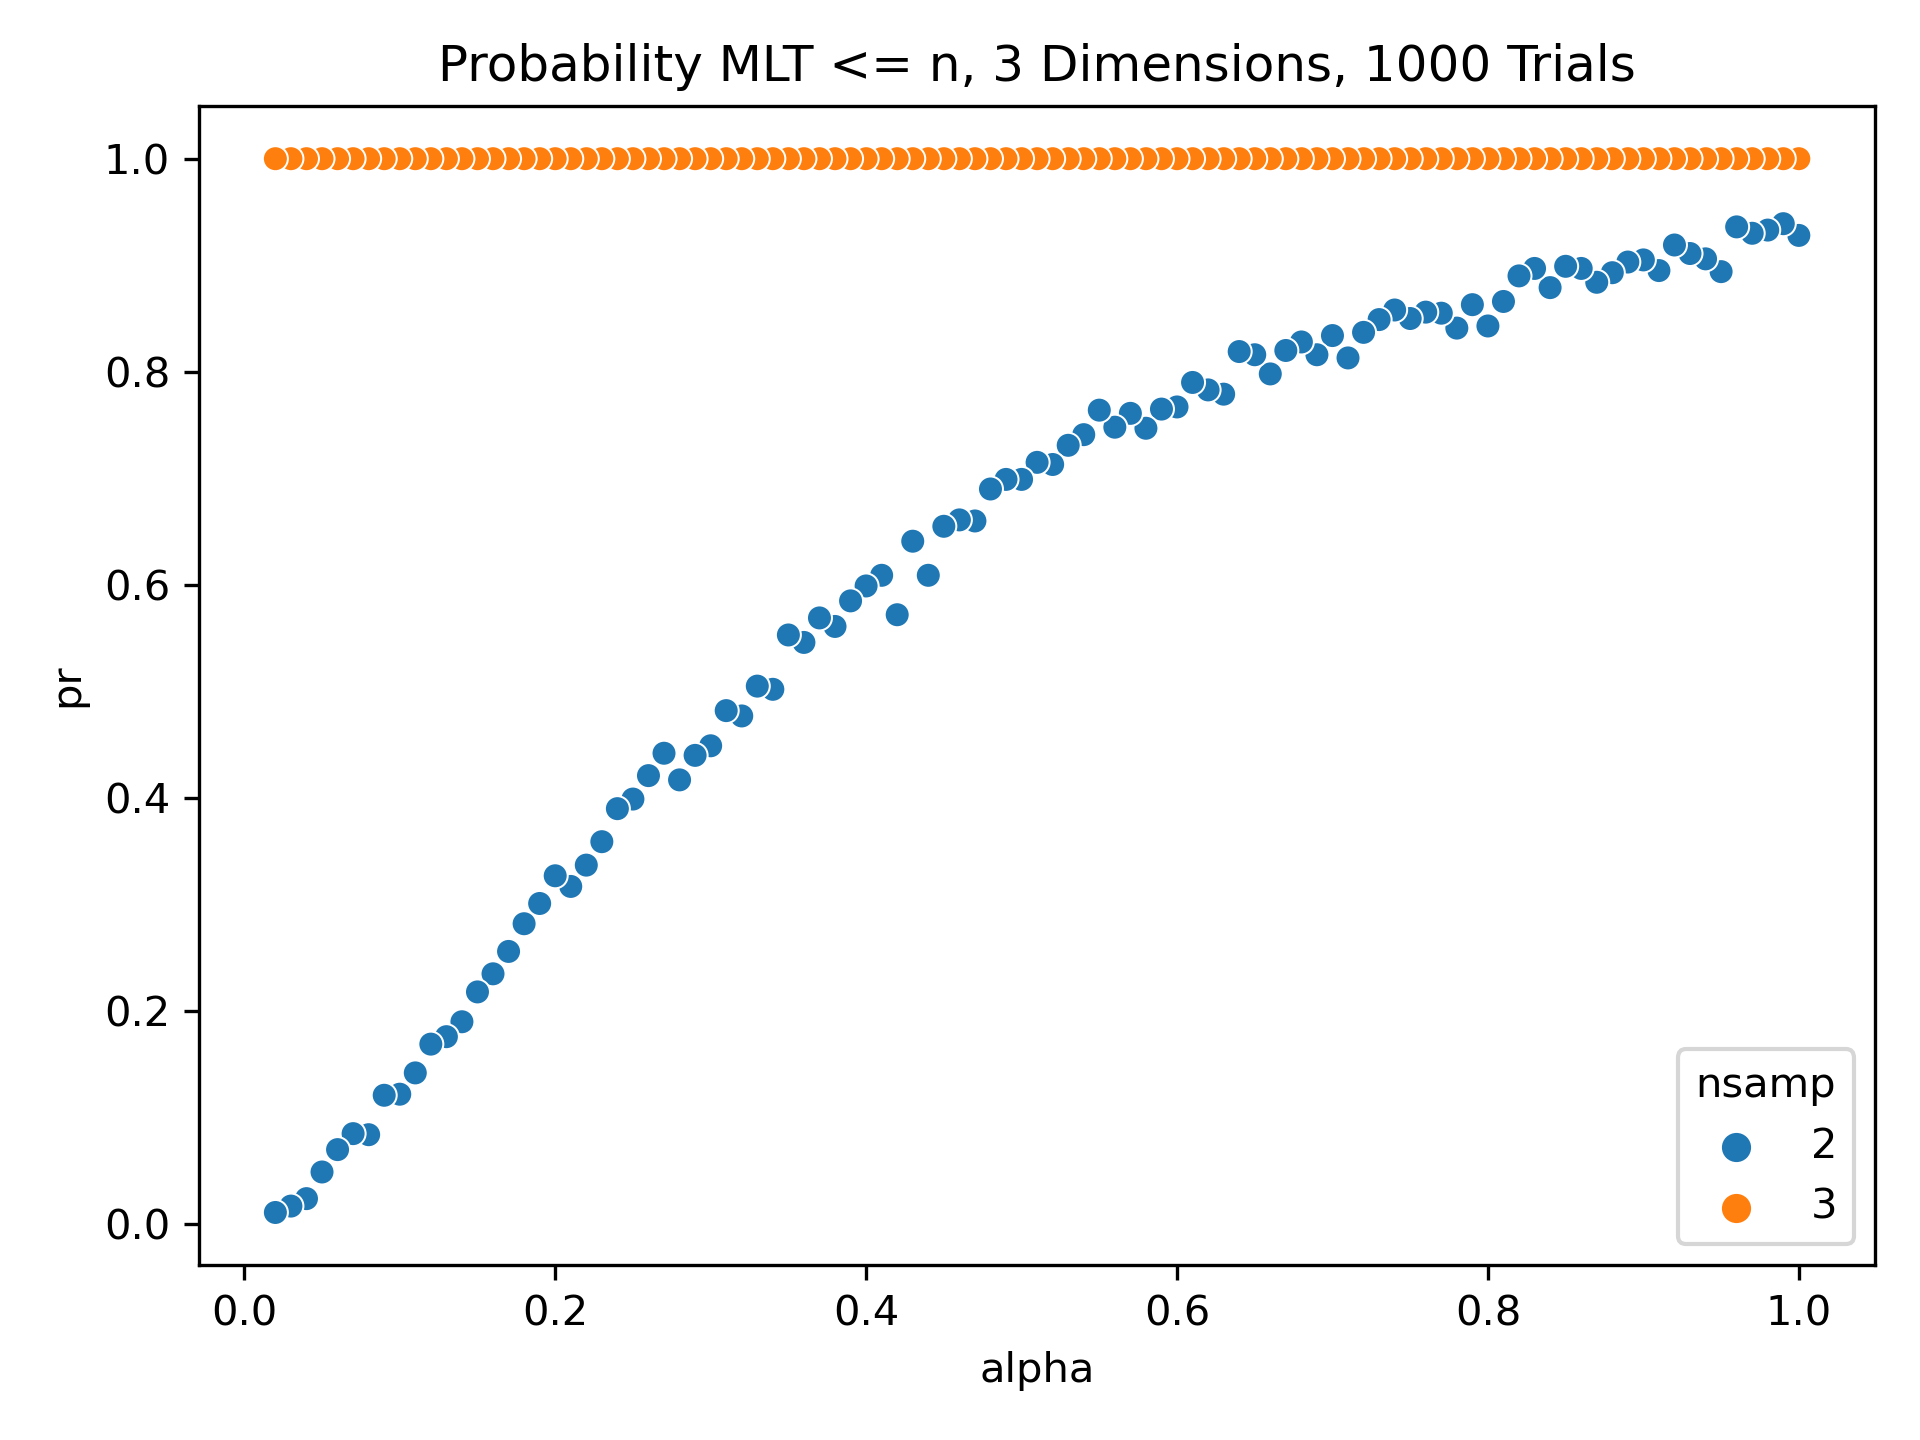
\includegraphics[width = 0.5\textwidth]{figures/3dPlot.png}
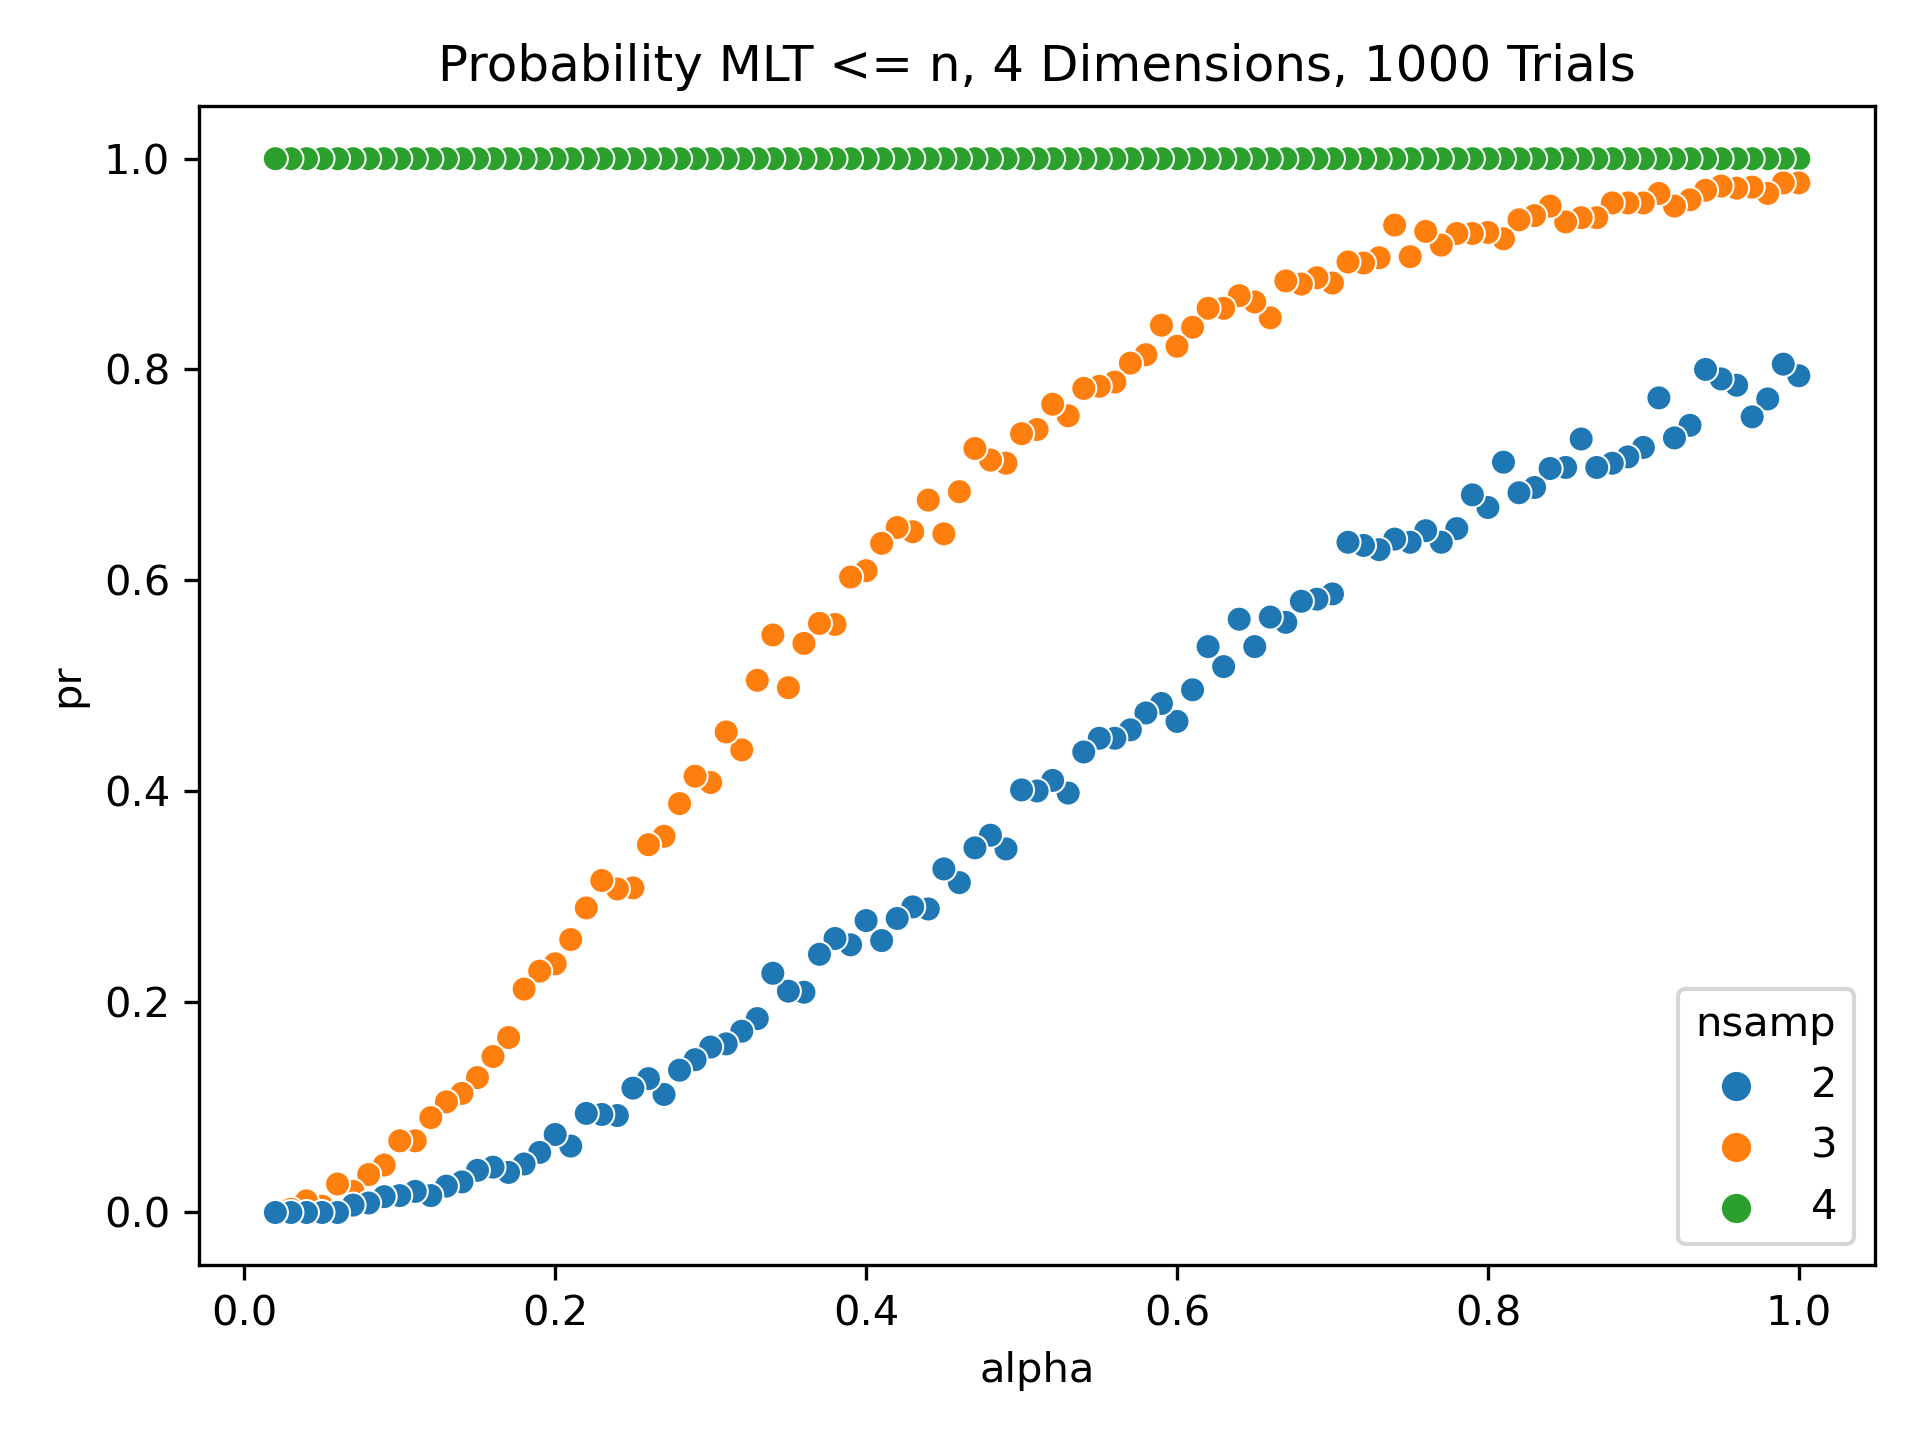
\includegraphics[width = 0.5\textwidth]{figures/4dPlot.png}
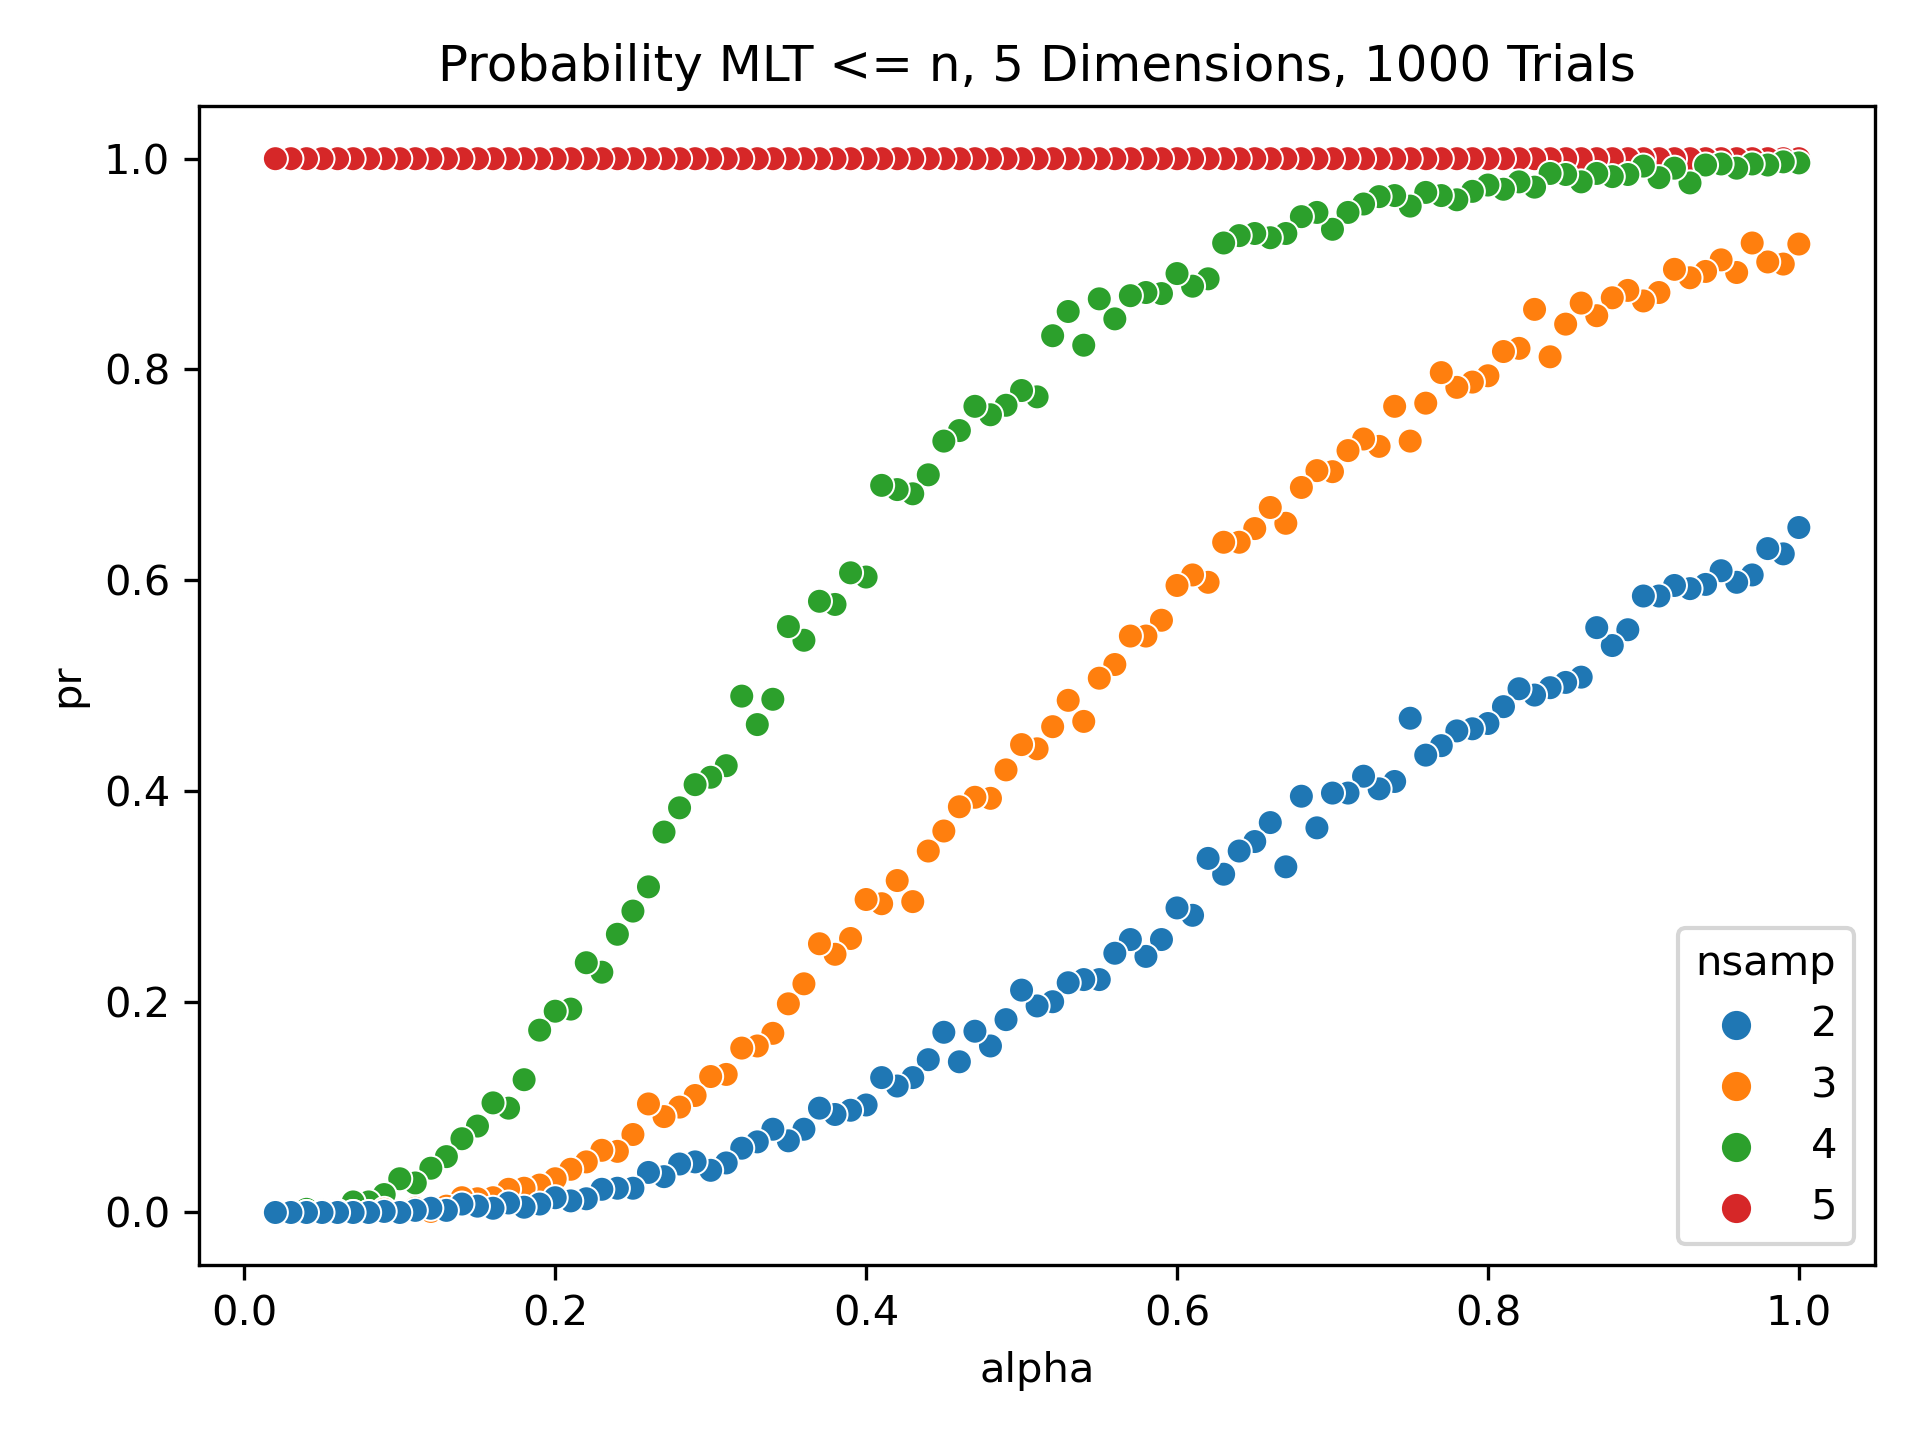
\includegraphics[width = 0.5\textwidth]{figures/5dPlot.png}
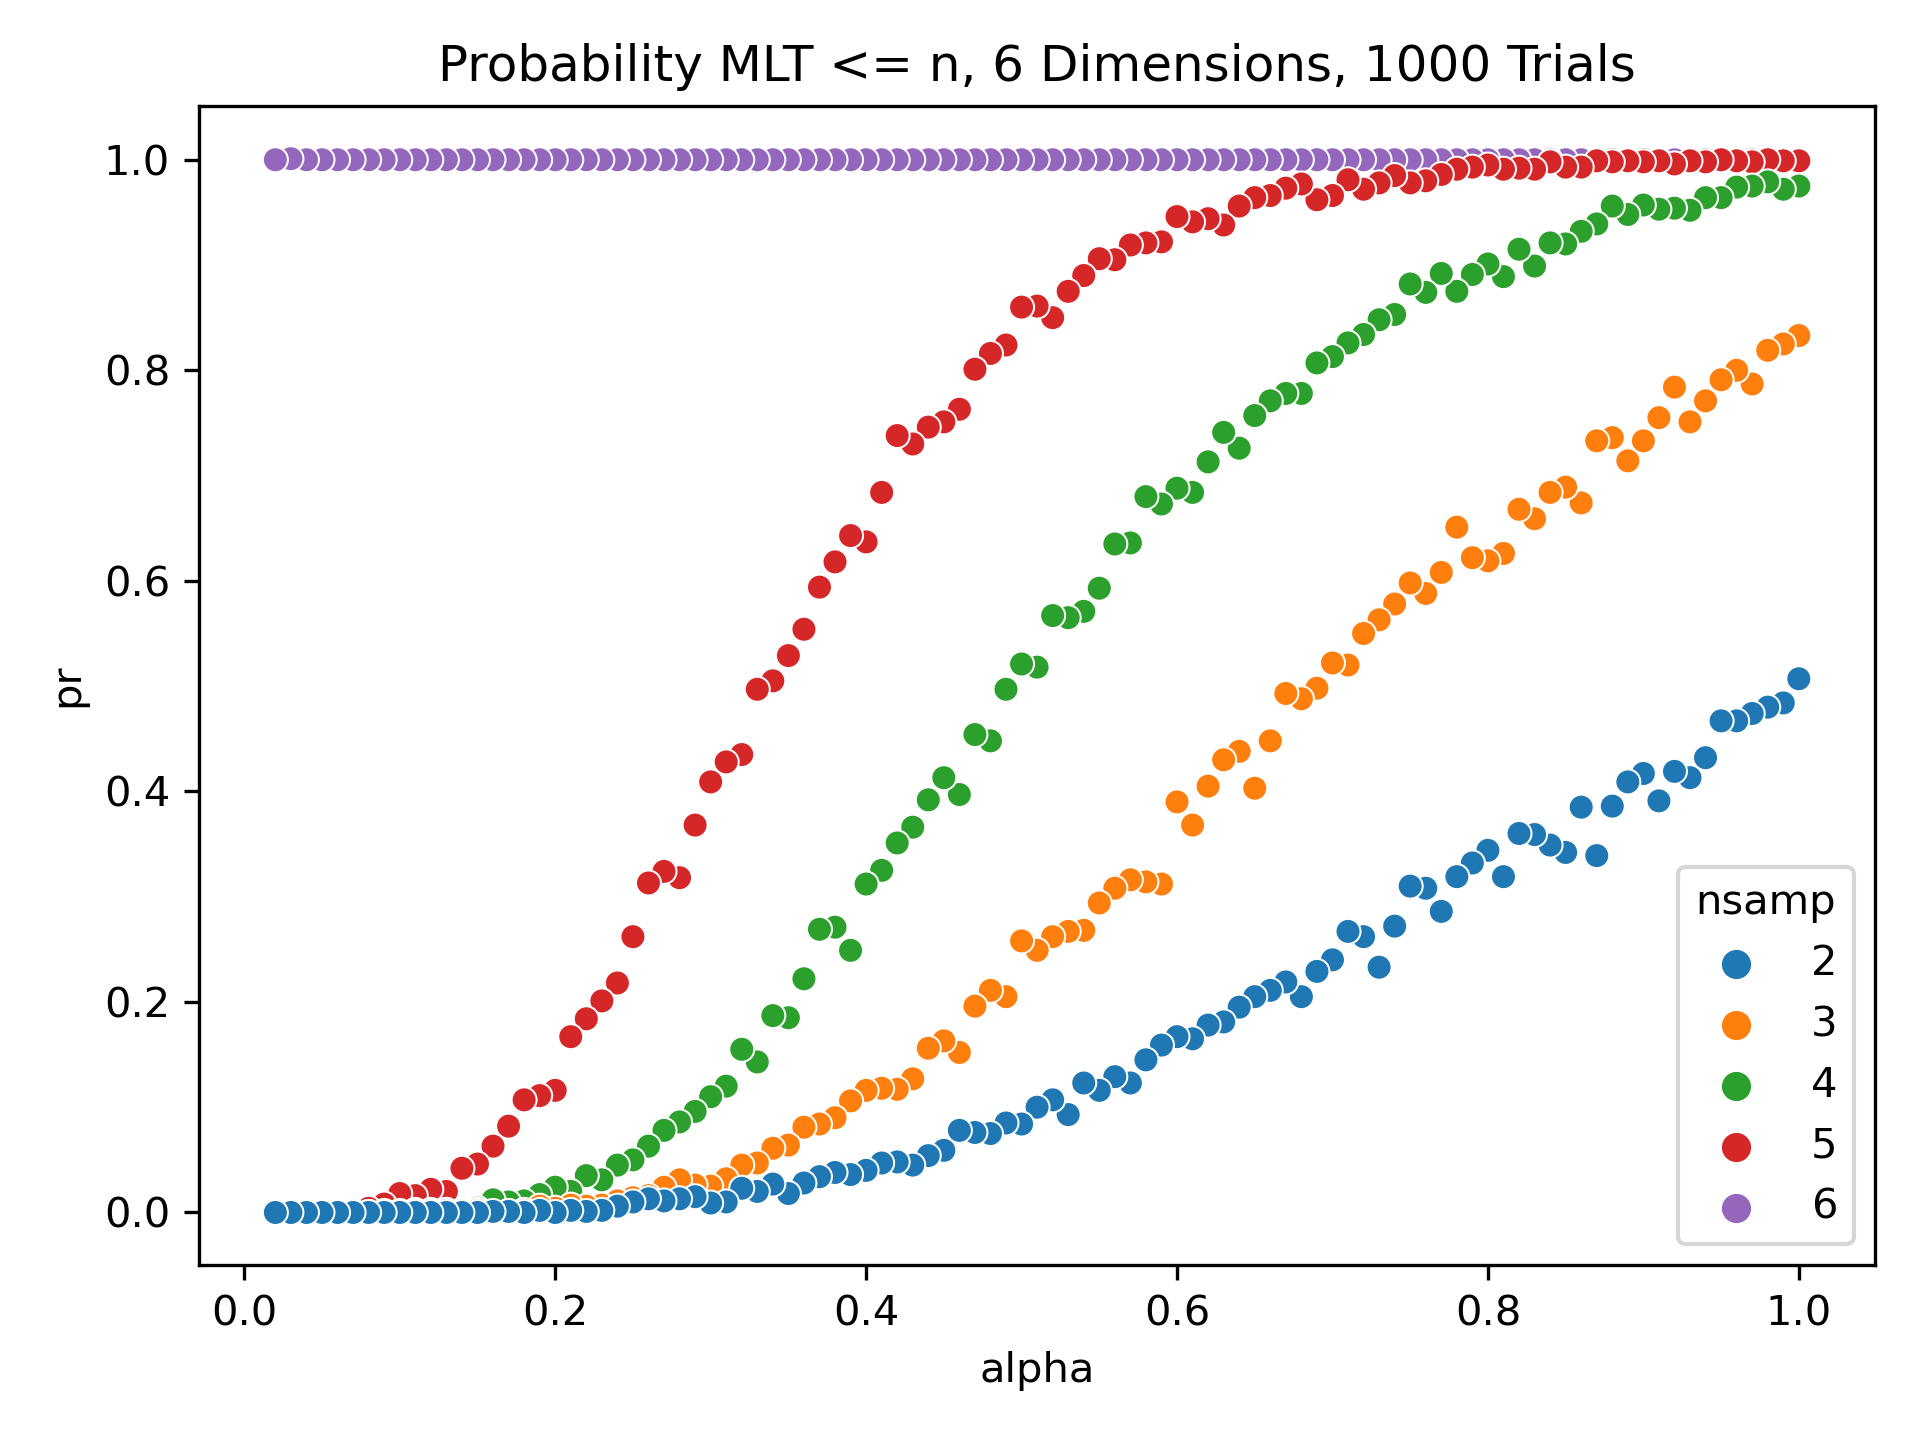
\includegraphics[width = 0.5\textwidth]{figures/6dPlot.png}
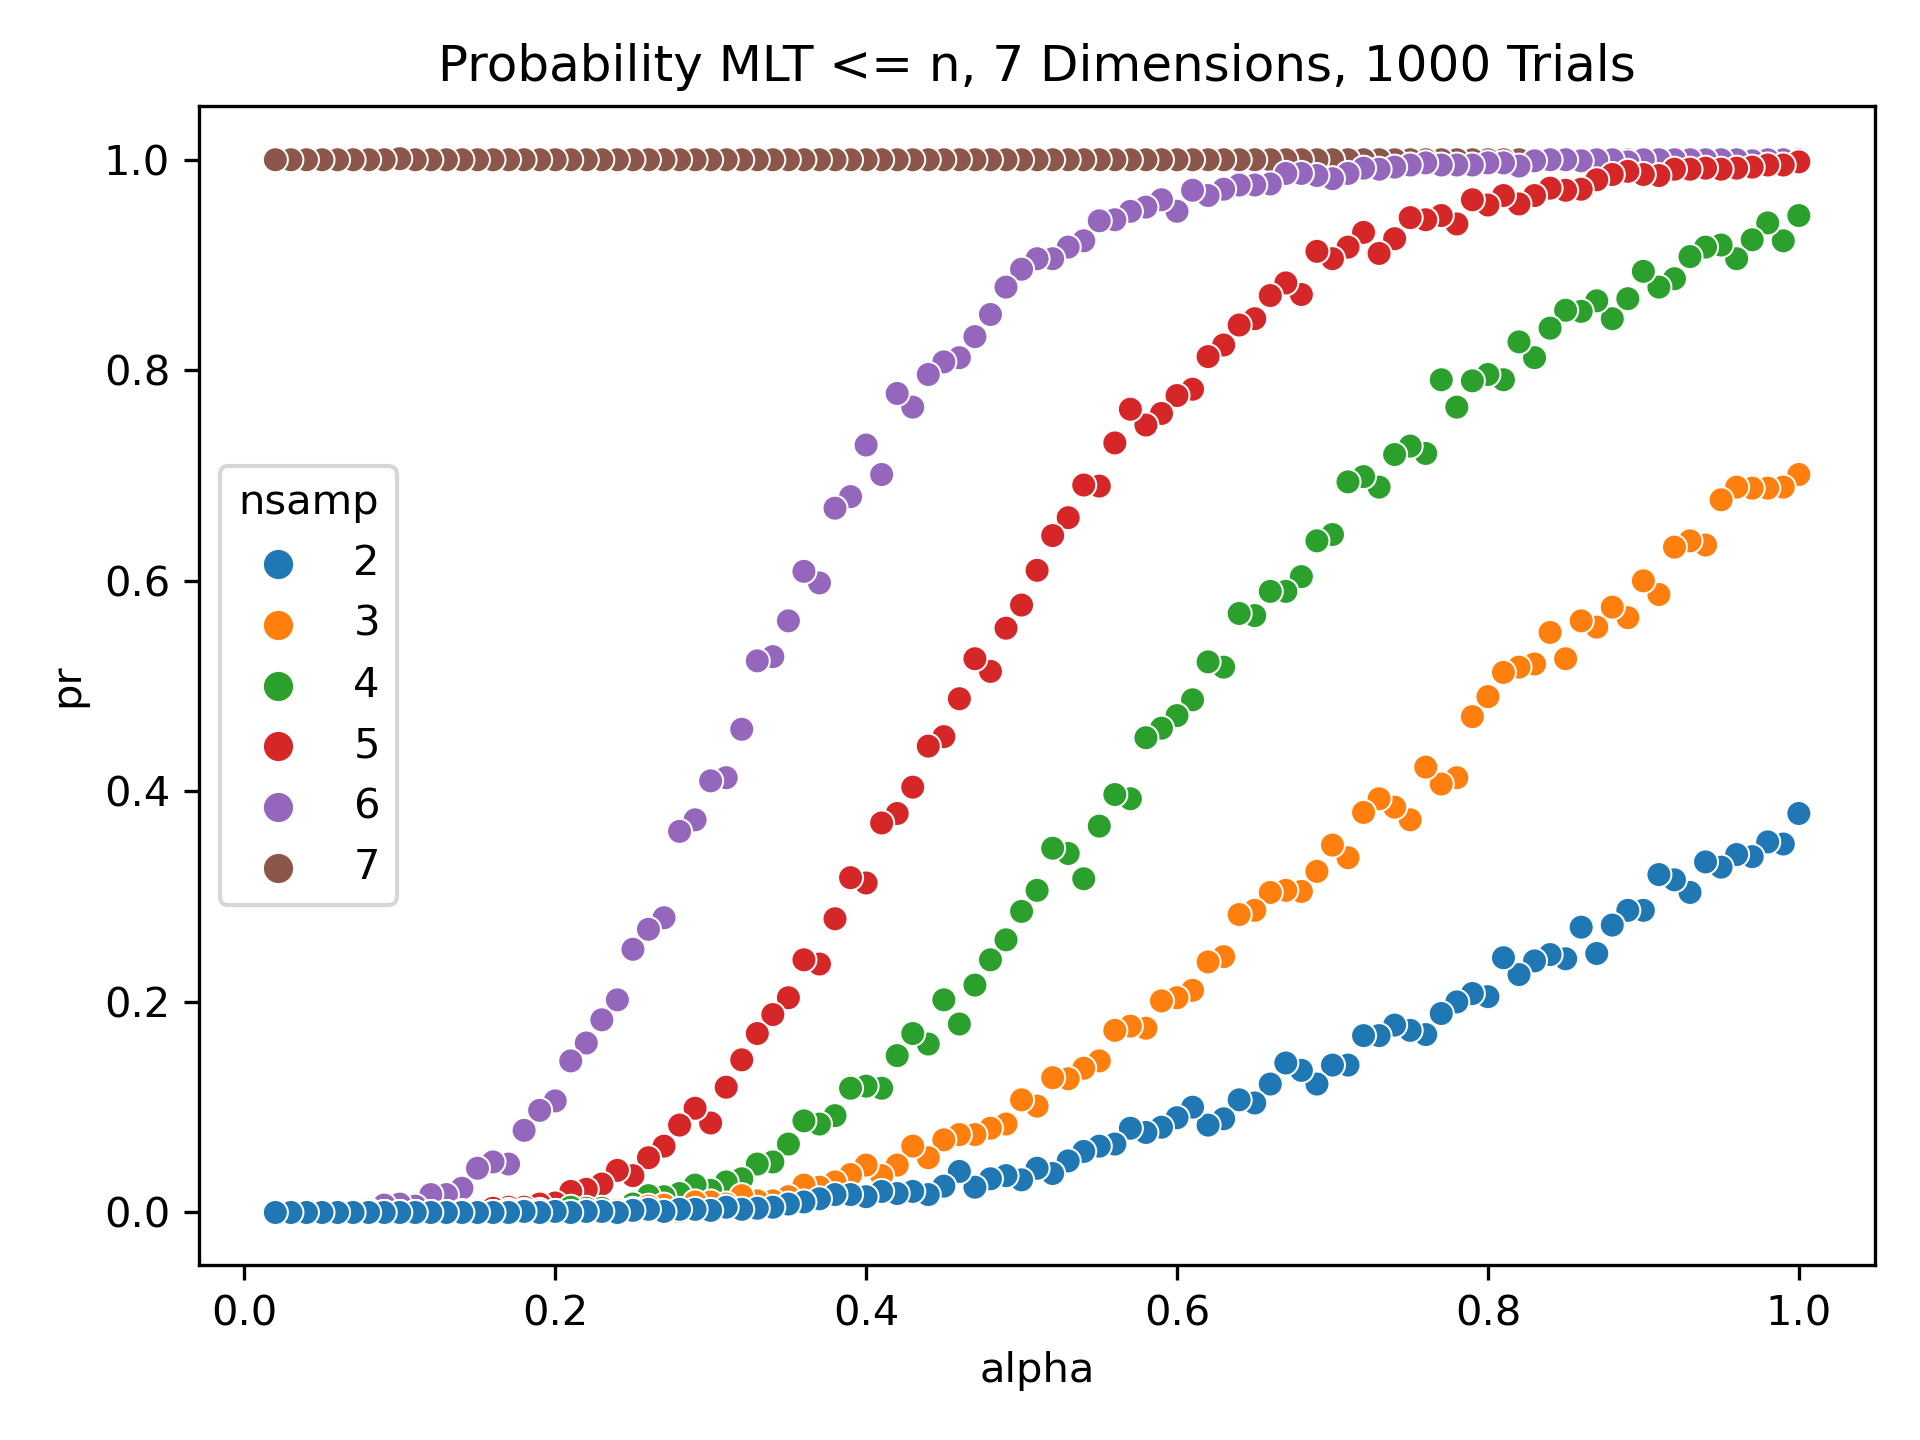
\includegraphics[width = 0.5\textwidth]{figures/7dPlot.png}
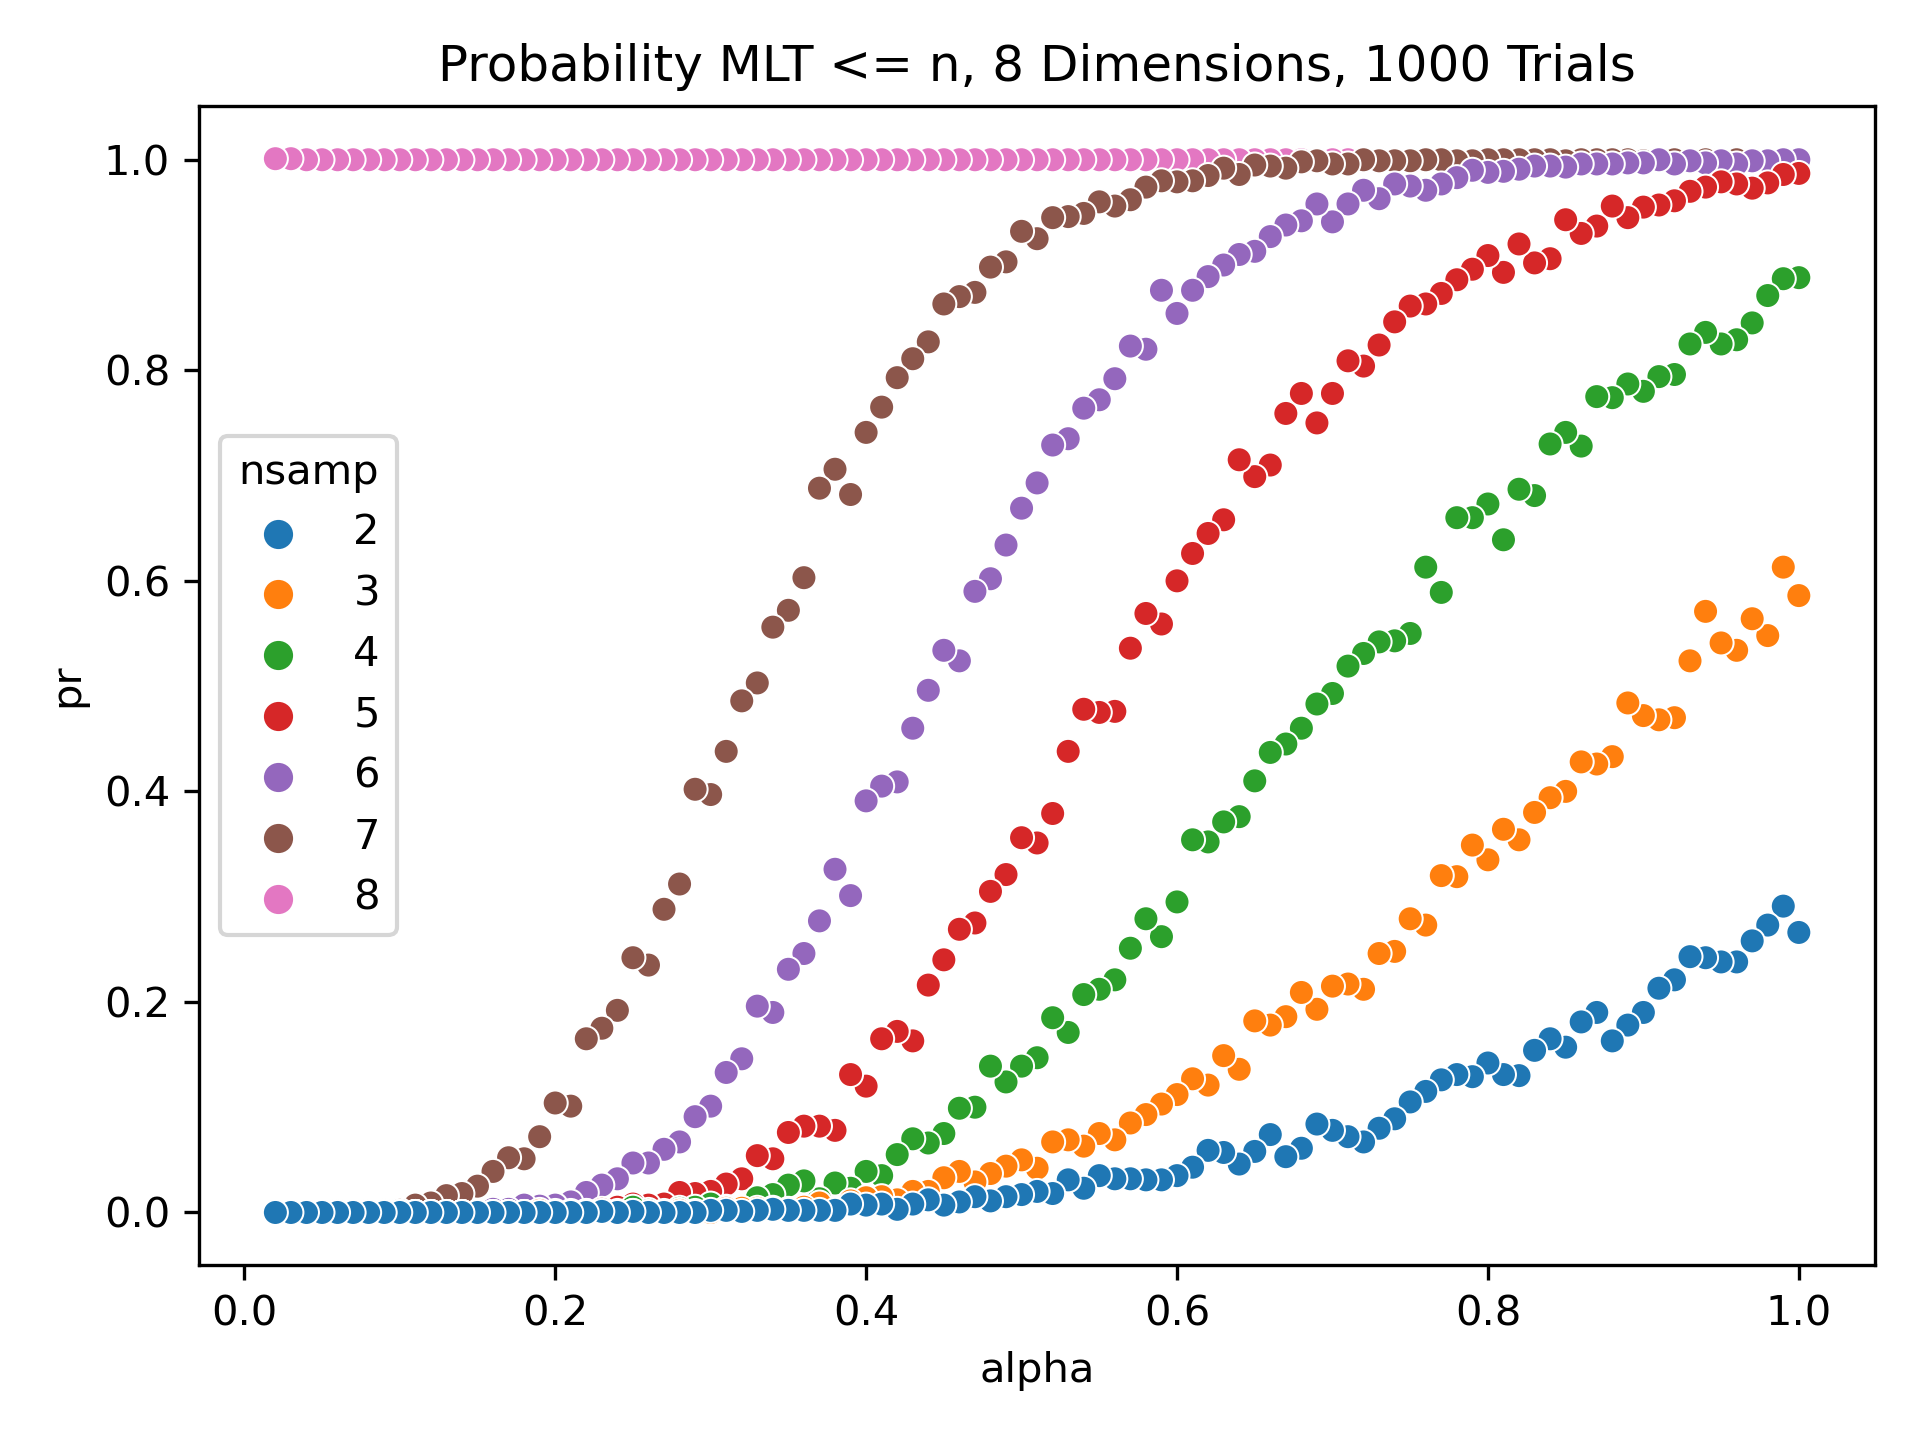
\includegraphics[width = 0.5\textwidth]{figures/8dPlot.png}
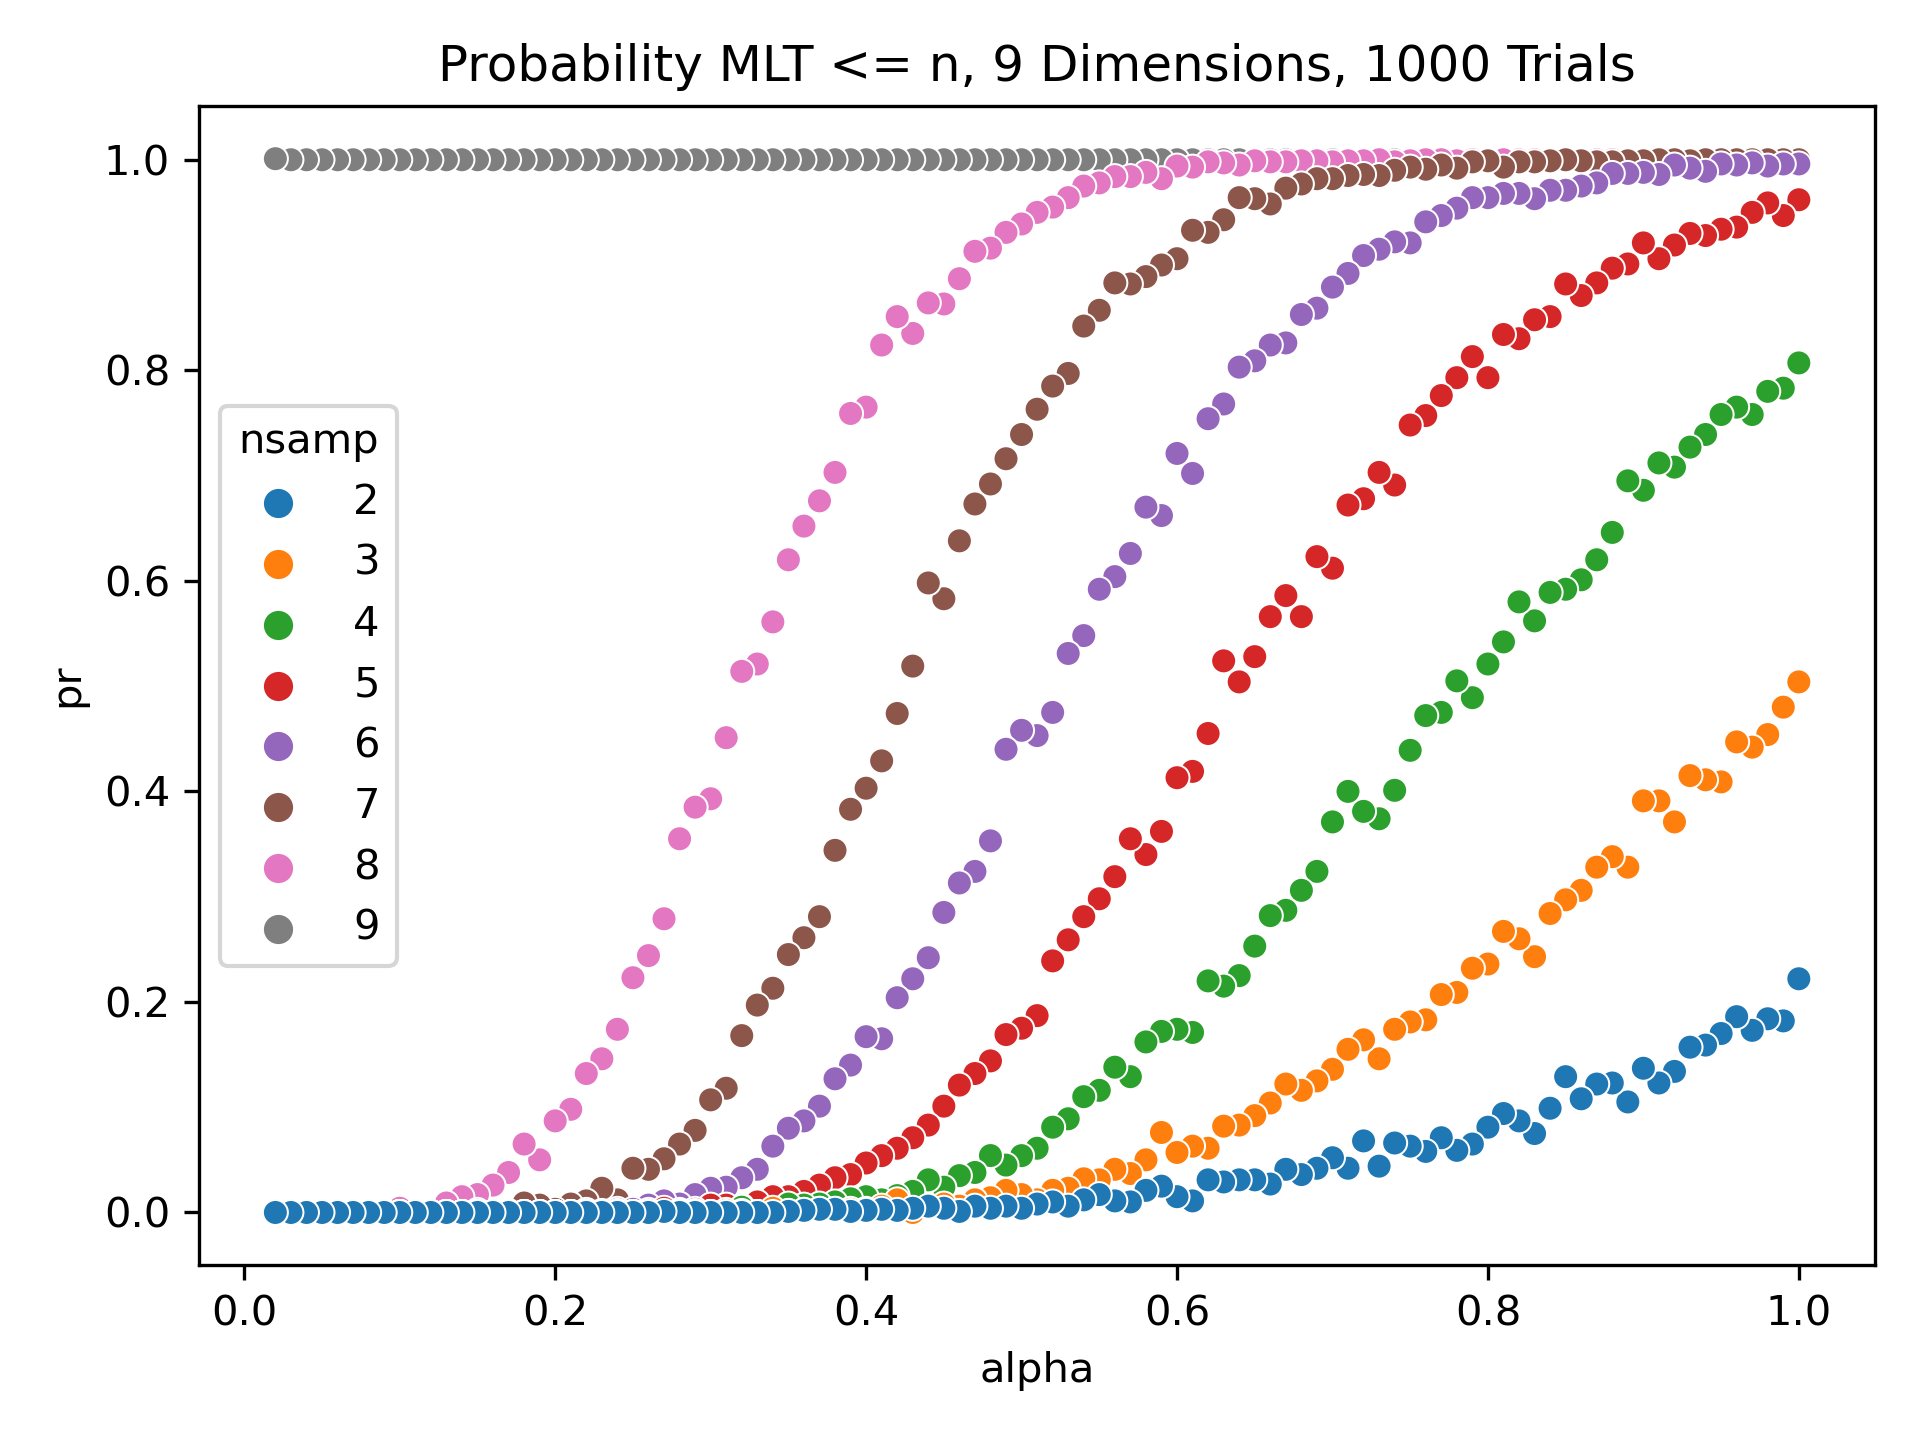
\includegraphics[width = 0.5\textwidth]{figures/9dPlot.png}

  \end{block}



\end{column}

\separatorcolumn

\begin{column}{\colwidth}

  \begin{block}{Discussion}
    For any given estimate $\hat{p}$, given that it is derived from $1000$ numerical samples, the confidence interval for the true value of $p$ can be assumed to be binomial according to $Bin(1000, p)$, and a $95\%$ confidence interval of the form $(\hat{p} \pm 1.96\sqrt{\frac{\hat{p}(1-\hat{p})}{1000}})$.

    Note that the MLT is upper bounded by the number of dimensions of the distribution - therefore, for all $n$ greater than or equal to the number of distribution, the probability that it is also greater than or equal to the MLT is $1$.
    
    From the large number of samples used in deriving $\hat{p}$, high fidelity curves were extracted from the numerical experiments. For each of the distributions for which the MLT could be calculated exactly, we were successfully able to model the relationship between the size of the sample and regularization quantity when the sample size was less than the number of dimensions. 

    To continue exploring this relationship, the next step would be to develop an analytical description of this relationship, as well as developing a mechanism for examining different distributions for which there only exist lower bounds on the MLT. 

  \end{block}

  


  \begin{block}{References}

    \nocite{*}
    \footnotesize{\bibliographystyle{plain}\bibliography{poster}}

  \end{block}

  \begin{block}{Acknowledgements}
    This project was funded and supported by the Tulane University Department of Mathematics.
  
  \end{block}

\end{column}

\separatorcolumn
\end{columns}
\end{frame}

\end{document}
